% Generated numerical fields are populated from the frozen-window and event ledgers.
\documentclass[10pt]{article}
\usepackage[margin=24mm]{geometry}\usepackage{amsmath,amssymb,graphicx,booktabs,tabularx,microtype,xcolor,hyperref}
\hypersetup{hidelinks}\setlength{\emergencystretch}{1.6em}
\title{When does short-window frequency shape improve early warning?\\ Decision deadlines, measurement noise and representation across simulated power systems}
\author{}\date{}
\begin{document}\maketitle\vspace{-2.8em}
\begin{abstract}
Short frequency records with nearly equal endpoints can precede different nadirs. Among 148 clean matched pairs, quadratic features reduced the mean absolute error of the predicted nadir difference by 4.89 mHz. In a prospective aggregate simulation with a 200-ms minimum lead, the full-window tree gained 35.14 percentage points [95\% interval 31.54, 38.57] in effective hits over a capacity-matched endpoint tree, at a false-alarm cost of 1.19 points [0.39, 1.99]. Direct transfer of the aggregate thresholds triggered no alarms on either target network. The historical IEEE 39 gain of 85.13 points under held readout compares fixed policies outside endpoint training support and cannot identify a physical shape effect: all 195 B variants received the same first-window endpoint-tree score. At a clock-aligned 1.25-ms step, the fixed policies alarmed on 54.50\% and 28.38\% of safe variants. In an independent test on 240 new IEEE 39 designs, both representations in both model families (boosted trees and ridge regression) warned in time on all 333 B variants. The full-window tree alarmed on 61/267 safe variants versus 33/267 for the endpoint, an excess of 10.49 points [2.53, 18.67]. The joint hit and false-alarm criterion failed. The same representation can improve timely warnings in the aggregate model and increase false alarms on a new network sample.
\end{abstract}
\noindent\textbf{Keywords}\quad frequency nadir, disturbance response, measurement quality, early warning, model transfer

\section{Introduction}
A frequency alarm issued during the initial decline must anticipate both how far frequency will fall and how soon it will cross a specified level. A model can estimate the eventual minimum accurately yet issue its first warning too late. A threshold that is effective on one system can also produce very different false-alarm rates on another. These two effects complicate the interpretation of gains attributed to richer inputs.

System frequency response models connect initial power imbalance to inertial and governor dynamics \cite{sfr,liu}. Short post-disturbance measurements have been used to predict the nadir with neural networks \cite{early}. Power--frequency polynomial fitting provides another route to predicting the minimum \cite{polynomial}. Transfer learning for frequency stability has already been evaluated on multiple benchmark networks using spatial and temporal measurements and network information \cite{transfer}. The scientific question here is narrower. For one scalar frequency channel, how much does the interior of the observed window contribute beyond its endpoint, when both predictors have the same opportunities, quality information and alarm budget? Which parts of that comparison survive a change of system?

Generator-bus voltage phase angles provide a complementary input for short-term nadir prediction \cite{nadir25}. A scalar frequency prefix poses a different identification question. Temporal detection metrics can depend on where within an event a detection occurs \cite{event}. We count an alarm only when its first occurrence leaves the specified lead time. Empirical false-alarm calibration also differs from a finite-sample guarantee on population type-I error \cite{calibration}. Our thresholds use an empirical safe-event quantile and we measure their realised cost on held-out designs.

Four questions guide the analysis. Can near-identical endpoints conceal predictable differences in the subsequent minimum? Can that information produce effective warnings before a fixed deadline? Does the gain require specialised residual compression, or can a quadratic fit or the raw prefix recover it? Finally, which part of a warning rule transfers: its threshold, its score function or its within-bin references?

We first isolate amplitude information by matching endpoints across different physical trajectories. We then change only the regressor input in a prospectively specified aggregate warning comparison. Finally we move the same predictors to two network models, replacing the operating threshold, the score function and the quality-bin references in sequence. A second, separately frozen network series changes the disturbance and inertia support to test when the first alarm can still be effective. The multi-machine experiments test a particular transfer direction and partially observed frequency response. They cannot establish a population effect across power networks.

\section{Endpoint constraints and shape representations}
In the aggregate experiment, $x$ is per-unit frequency deviation and $p$ is governor power. A deficit $d>0$ at $t=0$ drives
\[
 2H\dot x=-d-Dx+p,\qquad T_g\dot p=\mathrm{clip}(-x/R,0,0.1)-p .
\]
The clean initial state has $x=p=0$. For a short interval before the upper limiter binds, let $M=2H$ and subtract the endpoint chord $t x(\tau)/\tau$ from the trajectory. The residual is
\[
 \tfrac12 x''(0^+)(t^2-t\tau)+\tfrac16 x'''(0^+)(t^3-t\tau^2)+O(\tau^4),
 \quad x''(0^+)=Dd/M^2,\quad x'''(0^+)=-D^2d/M^3+d/(M^2RT_g).
\]
The first-order decline cancels. Damping and delayed governor response still affect the interior. This local expansion motivates the comparison without assigning a unique physical parameter to an estimated polynomial coefficient.

At 20-ms sampling, the fixed 0.50-s window contains 26 samples including its endpoint. Its target is the minimum strictly after the cutoff on the simulated trajectory. In the first retained matched pair, both endpoints round to 49.9204434 Hz. The subsequent minima are 49.89161 and 49.90161 Hz. Across the 148 eligible clean pairs, the endpoint and quadratic predictors gave within-pair difference errors of 11.64 and 6.75 mHz (mean absolute error). The paired change was $-4.89$ mHz (95\% interval $[-5.78,-3.92]$, resampling reference events within droop bands). This is evidence about the magnitude of a difference between trajectories. It does not count warnings.

\begin{figure}[ht]\centering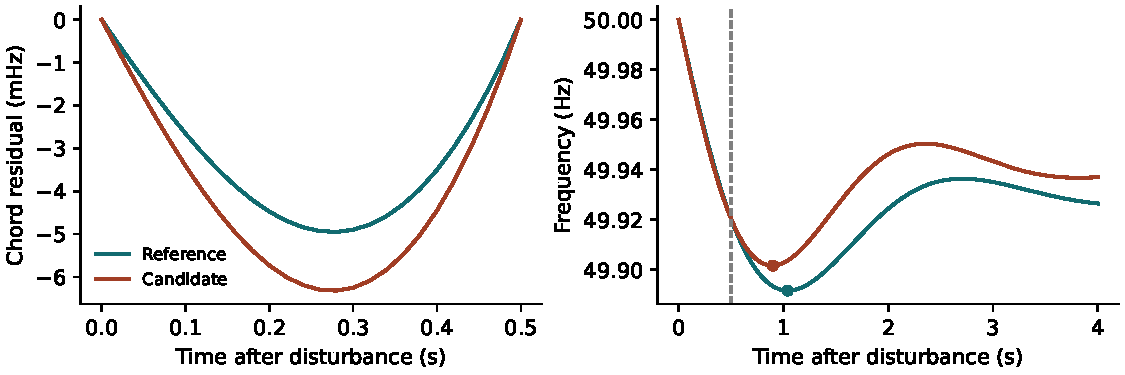
\includegraphics[width=.81\linewidth]{pair.pdf}
\caption{First eligible clean pair in archive order. The input endpoint is matched at 0.50 s. Subtracting the endpoint chord reveals the small difference in the visible shape; the two subsequent minima differ by 10.00 mHz.}\label{fig:pair}
\end{figure}
\paragraph{From the chord to a compressed representation.}
For a window of $n$ observations $f=(f_0,\ldots,f_{n-1})^\top$ in Hz, set $u_i=i/(n-1)$. Its interior residuals are
\[
 r_i=f_i-(1-u_i)f_0-u_i f_{n-1},\quad 1\le i\le n-2 .
\]
The two endpoints and all $n-2$ residuals reconstruct the whole window exactly. The endpoint-constrained, covariance-weighted chord-residual estimator (ECGR) compresses $r$ onto two columns evaluated at the interior samples: $u(1-u)$ measures symmetric bending, and $u(1-u)(2u-1)$ measures antisymmetric cubic bending. It whitens the residual and basis with the same working covariance and shrinks the cubic coefficient in proportion to unexplained variation. The predictor receives the final deviation and two coefficients. Compression changes how the tree can use the samples; it adds no measurement. The supplement gives the weighted objective, dimensions and frozen shrinkage rule.

The raw-window tree sees every deviation, the endpoint tree sees the last deviation, and persistence uses that last frequency directly without regression. The quadratic tree uses the endpoint plus the linear and quadratic terms of an unconstrained polynomial fit. A separate policy, the \emph{original gate}, uses $Q$ at each decision to select the ECGR predictor, the quadratic predictor or the endpoint predictor. Its first alarm can therefore originate from any of the three branches.

\section{Evidence hierarchy and frozen comparisons}
\begin{table}[htbp]\centering\small
\caption{Study lineage. Counts are physical units unless variants are stated. The fixed-cutoff and warning rows have different outcomes. Sources are the archived pair indices, earlier confirmation ledgers, and the aggregate and transfer protocols.}\label{tab:lineage}
\begin{tabularx}{\linewidth}{@{}p{.24\linewidth}X@{}}\toprule Evidence & Question and population\\\midrule
Historical development & Grid feature comparisons and quality-rule development selected representations. A separate clean matched-pair analysis (148 eligible pairs sharing reference scenes) tested amplitude differences.\\
Archive diagnostics & Component deletion reused pair predictions. Test-label equal-false-alarm curves and the older 118 solved IEEE 39 cases provide retrospective diagnostics.\\
First five-condition batch & Frozen gate versus ordinary persistence; 401 risk and 1,999 safe events, each with five variants. The raw-window contrast was post hoc.\\
Second five-condition batch & Frozen stratified window versus stratified persistence; 405 risk and 1,995 safe events. A trained endpoint comparison was added after inspection.\\
New three-condition batch & Sole prospective aggregate primary comparison: full window versus trained endpoint, 2,400 fresh events, three variants each. Other methods are secondary.\\
Original transfer series & Separate T3 tests on 600 planned designs per network. Each completed event has three variants. T0--T2 diagnose transfer stages.\\
Deadline study & New development support, training, calibration and 320 test designs per network. B-stratum full window versus endpoint is primary within each network.\\
r3 post hoc numerical-clock audit & Same 320 IEEE 39 test designs. Held and aligned reintegrations with historical trees, development offsets and thresholds. Identifies fixed-policy clock sensitivity only.\\
Independent support-stratified test & Fresh IEEE 39 pilot, training, development, calibration and test trajectories on aligned ticks. Refit and recalibrated before 240 test designs. Primary evidence for the new frame: full versus endpoint tree on B, with a common safe-event cost guard.\\\bottomrule
\end{tabularx}\end{table}

\paragraph{Readout scope.} The aggregate RK4 code stores the initial state and every fourth accepted 5-ms step. A traced archive design reproduced the 26 clean readings used through 0.50 s. The original network transfer ladder and all four deadline-study splits sampled the last accepted state at each nominal 20-ms tick. In the numerical audit, held runs varied the solver while retaining that rule, and aligned runs constrained the solver to reach each tick. Both reused the historical trees, development offsets and calibration thresholds. Only the independent support-stratified study regenerated every split on aligned ticks and fitted and calibrated fresh policies.

\paragraph{Aggregate confirmation.}
The two scores predict the minimum strictly after each of four decision times, 0.20, 0.30, 0.40 and 0.50 s. One boosted tree ensemble per time uses the last deviation; its counterpart uses all deviations up to and including that time. Both used the same 1,200 clean training trajectories, targets and hyperparameters (100 boosting stages, maximum depth three). The common quality proxy $Q$ combines the variability of 50 pre-disturbance samples and the third differences of the visible window, normalised by a common amplitude estimate. Both scores thus have indirect access to a roughness statistic. The comparison identifies the added value of supplying the whole waveform beyond the endpoint \emph{and} this shared proxy.

Each score has separate quality-bin references estimated from 800 development events and a separate global threshold calibrated on another 800 events. Both use the same three bins and the same event-level 10\% false-alarm target. Only safe calibration events determine thresholds. We froze model files, binary thresholds, code, sample size, seeds, lead time and acceptance limits before generating the 2,400 confirmation events. Each clean trajectory has three equally weighted variants: clean, white noise, and stationary AR(1) noise with coefficient 0.8. Both noises have standard deviation 0.003 Hz on the common 50-Hz scale. This absolute noise law can be specified before a disturbance. Earlier event-relative noise trials are reported separately in the supplement.

\paragraph{Endpoints and uncertainty.}
A risk event first crosses below 0.995 pu on the 20-ms truth grid. The first score strictly below its threshold issues the only alarm. An effective hit must precede crossing by at least 200 ms. Every risk event contributes to the denominator, including those crossing before any valid alarm is possible. A false alarm is any first alarm on a safe event. The risk level is an experimental outcome definition. The score threshold is a calibrated policy parameter. Neither specifies a field load-shedding setting. The primary difference (full window minus endpoint) must have a positive 95\% lower bound for effective hits and a 95\% upper bound no greater than two percentage points for additional false alarms. We compute paired percentile intervals from 2,000 bootstrap samples of physical events, carrying all measurement variants together. The limits are marginal; finite calibration and training sets are held fixed.

\paragraph{Multi-machine cases.}
We used the ANDES time-domain simulator \cite{andes}. The Kundur case has 10 buses, four synchronous machines and two areas; the New England case has 39 buses and ten synchronous machines. We scaled initial active and reactive demands together, solved power flow and applied a load increase at 1 s. The predictor observes the unweighted mean of three bus-frequency channels. Risk and target magnitude use inertia-weighted synchronous-machine speeds. We express 60-Hz outputs on a 50-Hz equivalent scale for source-model inference, preserving the per-unit risk definition. No system identity, contingency magnitude, inertia or future sample enters the scores.

Small-step and backward-Euler checks preceded an unscored 100-design pilot on each system. The pilot informed two site-specific disturbance ranges and a fixed design budget of 240 training, 120 development, 180 calibration and 600 confirmation designs per network. Splits have separate seeds and no shared physical parameter tuple within a network. Incomplete simulations retain unknown risk. The reported operating rates condition on complete 21-s solutions. Supplementary material gives the full ledger, operating ranges, numerical checks and worst-case missing-event bounds.

\begin{table}[ht]\centering\small
\caption{Transfer protocol for the two network tests (600 physical designs each; three variants per completed design). What changes at each level. The waveform input, bin boundaries, alarm rule and 200-ms deadline stay fixed.}\label{tab:levels}
\begin{tabular}{llll}\toprule Level & Scoring function & Bin references & Global threshold\\\midrule
T0 & Aggregate & Aggregate & Aggregate\\
T1 & Aggregate & Aggregate & Target calibration\\
T2 & Target training & Aggregate & Target calibration\\
T3 & Target training & Target development & Target calibration\\\bottomrule
\end{tabular}\end{table}
Both local trees fit the same three variants of each target training event. T2--T3 therefore isolates a change of bin references with the score functions held fixed and the global threshold recalibrated. At each network the single primary comparison is the T3 full-window versus endpoint contrast. The other levels, persistence, quadratic predictors and individual measurement strata are supporting comparisons. We require both networks to pass before claiming a shared local shape benefit.

\section{Aggregate warning results}
\begin{table}[ht]\centering\small\caption{Frozen operating points under equal weights (count and paired ledgers). In each system the difference is full window minus endpoint. Additional aggregate methods are secondary. Denominators are risk and safe combinations, three per completed event. Network rows use T3. Differences and clustered intervals are in percentage points (pp).}\label{tab:primary}
\begin{tabular}{llrr}\toprule System & Score & Effective hits & False alarms\\\midrule
Aggregate & Endpoint & 313/1215 & 552/5985 \\
Aggregate & Persistence & 428/1215 & 512/5985 \\
Aggregate & Original gate & 645/1215 & 565/5985 \\
Aggregate & Quadratic & 737/1215 & 666/5985 \\
Aggregate & Full window & 740/1215 & 623/5985 \\
 & Difference (pp) & 35.14 [31.54, 38.57] & 1.19 [0.39, 1.99] \\\addlinespace
Kundur & Endpoint & 560/600 & 144/960 \\
Kundur & Window & 575/600 & 115/960 \\
 & Difference (pp) & 2.50 [1.10, 3.98] & -3.02 [-4.99, -1.20] \\\addlinespace
IEEE 39 & Endpoint & 217/336 & 98/1425 \\
IEEE 39 & Window & 315/336 & 112/1425 \\
 & Difference (pp) & 29.17 [23.96, 34.41] & 0.98 [-1.17, 3.05] \\\addlinespace
\bottomrule\end{tabular}
\end{table}
In the aggregate confirmation, 405 events crossed the risk level and 1,995 remained above it. The full-window method gained 427 effective hits and incurred 71 additional false alarms (Table~\ref{tab:primary}). The unrounded false-alarm upper bound was 1.9879 pp, a narrow pass. Acceptance therefore depends on the specified two-point tolerance. The result does not demonstrate equivalence of false-alarm rates. Quadratic features yielded 737 effective hits and 666 false alarms, compared with 740 and 623 for the raw window. Their similar hit counts make it difficult to attribute the aggregate benefit to a particular complex shape estimator.

\section{Representation diagnostics}
On the archived fixed-cutoff pairs, removing the cubic term changed clean MAE/P95 from 4.44/11.20 to 4.29/12.37 mHz: mean error fell while tail error rose. With 30-dB white noise, removing whitening raised MAE/P95 from 13.96/39.57 to 19.64/54.04 mHz. Even the full estimator exceeded its historical 36.04-mHz tail limit. Those errors concern predicted differences between paired minima. They cannot be assigned to the four-window switching policy.

In the new aggregate comparison the original gate issued 645 effective warnings and 565 false alarms. It produced fewer of both than the full window. Neither the aggregate count nor a count within a noise stratum identifies which branch would have prevailed if used throughout. The following secondary operating points show how the policy changes position relative to the simpler representations.
\begin{table}[htbp]\centering\small
\caption{Aggregate representation diagnostics from the frozen event ledger. Each condition contains the same 405 risk and 1,995 safe physical events; each cell gives effective hits / false alarms, with one variant per event.}\label{tab:strata}
\begin{tabular}{lrrr}\toprule Score or policy & Clean & White & AR(1)\\\midrule
Endpoint & 95 / 179 & 111 / 182 & 107 / 191 \\
Persistence & 146 / 172 & 140 / 176 & 142 / 164 \\
Original gate & 343 / 70 & 151 / 248 & 151 / 247 \\
Quadratic & 367 / 192 & 177 / 227 & 193 / 247 \\
Full window & 251 / 196 & 255 / 210 & 234 / 217 \\
\bottomrule\end{tabular}\end{table}
\paragraph{Measurement conditions.}
Relative to the endpoint, full-window effective hit rates increased by 38.52, 35.56 and 31.36 pp for clean, white and correlated measurements. Corresponding false-alarm costs were 0.85, 1.40 and 1.30 pp. Both noisy strata had upper false-alarm bounds above two points, although the equal-weight primary comparison passed. Under clean measurements the quadratic predictor yielded 367 hits to the raw window's 251; under white and correlated noise it yielded 177 and 193 to the raw window's 255 and 234. The representation ranking thus depends on the measurement law even within the same physical simulator.

\section{Cross-system transfer on the original disturbance support}
The prespecified target comparisons concern the raw-window and endpoint trees. This transfer series tested neither a transported ECGR nor a transported original gate. The subsequent deadline study fits their component scores locally. On Kundur, the T3 full-window minus persistence differences were $+1.33$ [$-0.20$, 2.92] pp for effective hits and $-0.42$ [$-2.32$, 1.45] pp for false alarms. These intervals establish no advantage over persistence.

At T0, none of the four rules fired on any completed target event, including late alarms. Replacing the global threshold (T1) yielded 551/600 effective hits and 112/960 false alarms for the full window on Kundur, compared with 555 and 81 for the endpoint. Source scores retained discrimination there: their deadline-aware AUCs were 0.962 and 0.981. Recalibration restored operation without establishing a shape advantage. After target training (T2), the window gained 15 hits and avoided 29 false alarms relative to the endpoint (Fig.~\ref{fig:ladder}). At T3 the achieved false-alarm rates were 11.98\% for the window and 15.00\% for the endpoint, despite a shared 10\% calibration target. Passing the relative-cost guard therefore does not certify an absolute 10\% operating rate. T2 and T3 produced identical first alarms on every Kundur variant. The effect of transferring quality-bin references is therefore unidentifiable on this network. All 6,240 window visits, including clean measurements, occupied the highest-$Q$ bin. Within one occupied bin, an additive reference is absorbed by independent global threshold calibration.

On IEEE 39, T1 recovered 169/336 effective hits for the window and 13/336 for the endpoint, with 98 and 113 false alarms among 1,425 safe variants. The source window therefore retained useful ordering at a locally chosen threshold. At T2, window hits rose to 312/336 with 103 false alarms; the descriptive window AUC rose from 0.884 to 0.978. Both the absolute threshold and the source score relationship limited direct performance. At T3, locally estimated bin references raised endpoint hits to 217 and window hits to 315. The primary hit contrast remained positive. Its accompanying false-alarm cost was 0.98 pp, with an upper bound of 3.05 pp. The favourable T1 contrast is a secondary result and cannot replace this failed primary guard.
\begin{figure}[ht]\centering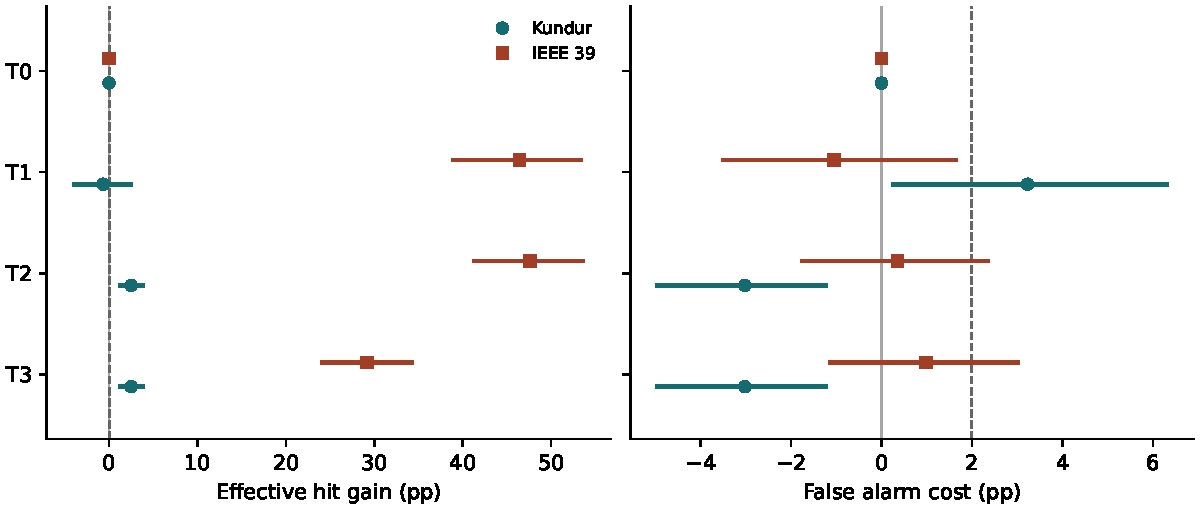
\includegraphics[width=.94\linewidth]{ladder.pdf}
\caption{Full-window minus endpoint differences on the same completed target events. Bars show event-clustered 95\% intervals. Dashed lines mark the primary boundaries (zero pp for hits, two pp for false-alarm cost). T0--T2 give secondary contrasts.}\label{fig:ladder}
\end{figure}
The network averages conceal different noise responses. On Kundur the T3 window gained 6.00 pp in clean effective hits and 1.00 and 0.50 pp in white and correlated noise; both noisy hit intervals included zero. On IEEE 39 the gains were 5.36, 43.75 and 38.39 pp. Correlated noise raised false alarms from 41 to 63 among 475 safe events ($+4.63$ pp, interval 1.08 to 8.04). The median lead times among effective hits, full per-condition counts and paired comparisons with persistence are in the supplement. Quadratic fits recorded 579 versus 575 full-window hits on Kundur and 311 versus 315 on IEEE 39; the corresponding false alarms were 136 versus 115 and 129 versus 112. These comparisons do not establish equivalence or a need for a more elaborate estimator.

\section{Warning opportunity on a new disturbance support}
A warning at time $t$ is effective when $t\leq b-200$ ms. A crossing before 400 ms (A) leaves no admissible alarm. For $400\leq b<700$ ms (B), the 500-ms decision is too late. For $b\geq700$ ms (C), all four decisions are eligible. The first crossing $b$ is scored on the 20-ms COI grid after simulation. The online models see the bus-frequency prefix and the common quality proxy.

A numerical development grid changed the distribution of the load step and scaled synchronous inertia. Each network supplied four scenario cells chosen by opportunity and solver support before any warning scores were examined. The formal draws sample these cells uniformly, with continuous load and step jitter. Their proportions describe this experimental design. Crossing time, inertia and perturbation size vary together, so a difference between strata cannot isolate the causal effect of moving a deadline. Each network had separate training, quality-reference development, safe-event calibration and test draws (180, 112, 220 and 320 designs). Only complete training trajectories supplied suffix minima. A failed test trajectory can supply a known crossing and every earlier opportunity needed to evaluate an effective alarm. Safety requires the complete 20-s horizon.

The endpoint, quadratic, raw-window and ECGR trees have the same boosting budget, training targets and four decision times. Persistence returns the latest observation. The locally fitted original switch uses the historical $Q$ cutoffs to select the ECGR, quadratic or endpoint prediction, in that order as $Q$ increases. All six policies receive the same per-bin reference procedure and a single method-specific threshold from safe calibration events. The switch consequently tests the historical selection rule within the common local calibration procedure. It is a separate policy from ECGR. The complete rules were frozen before drawing the test designs.

We prespecified one comparison per network on the new support. For full window minus endpoint the B-stratum hit interval had to lie above zero and the upper limit on the safe-event false-alarm cost had to be at most two percentage points. B minus C and the three measurement-specific contrasts are prespecified secondary analyses in this series. Each bootstrap draw retains all variants of a physical event. Intervals condition on realised class, observed outcomes and fitted rules.

Kundur had 38, 84, 75, 82, 41 designs in A, B, C, safe and unknown order. The B-minus-C hit contrast was 0.00 [0.00, 0.00] percentage points. Kundur did not meet both limits.

IEEE 39 had 85, 65, 96, 74, 0 designs in A, B, C, safe and unknown order. Resampling the 65 B and 96 C designs separately gave a B-minus-C hit contrast of 85.13 [76.76, 92.99] percentage points. IEEE 39 did not meet both limits.
\begin{table}[htbp]\centering\small
\caption{Paired full-window minus endpoint rate differences in points [event-clustered 95\% interval]. Each design contributes three variants. B and C intervals resample designs within each stratum; Tables~\ref{tab:r2time} and~\ref{tab:r3clock} resample all 320 designs and recompute the B denominator. Safety cost uses the common safe designs.}\label{tab:new-contrast}
\begin{tabular}{@{}llll@{}}\toprule
Network & B hits & C hits & Safe alarms \\\midrule
Kundur & 0.00 [0.00, 0.00] & 0.00 [0.00, 0.00] & -1.63 [-6.10, 2.85] \\
IEEE 39 & 85.13 [76.92, 92.82] & 0.00 [-1.04, 1.04] & -0.45 [-4.97, 4.50] \\
\bottomrule\end{tabular}\end{table}

The two strong alternatives change the interpretation of any endpoint advantage. Kundur B-stratum hit differences for the full window were 100.00 [100.00, 100.00] points against persistence and 0.00 [0.00, 0.00] against the quadratic representation. IEEE 39 B-stratum hit differences for the full window were 85.13 [76.92, 92.82] points against persistence and 87.69 [83.08, 91.79] against the quadratic representation. Figure~\ref{fig:conditions} shows that the three measurement laws can be compared within each system and crossing stratum, with a common safe population below. The supplement gives first-alarm times and effective leads. A safe event has no crossing stratum. To examine the decision-time cost on the same safe events, we stop accepting first alarms successively after 200, 300, 400 and 500 ms. Kundur full-window minus endpoint false-alarm costs at the first and last of these horizons were 1.63 and -1.63 points. IEEE 39 full-window minus endpoint false-alarm costs at the first and last of these horizons were 8.11 and -0.45 points. 
\begin{figure}[htbp]\centering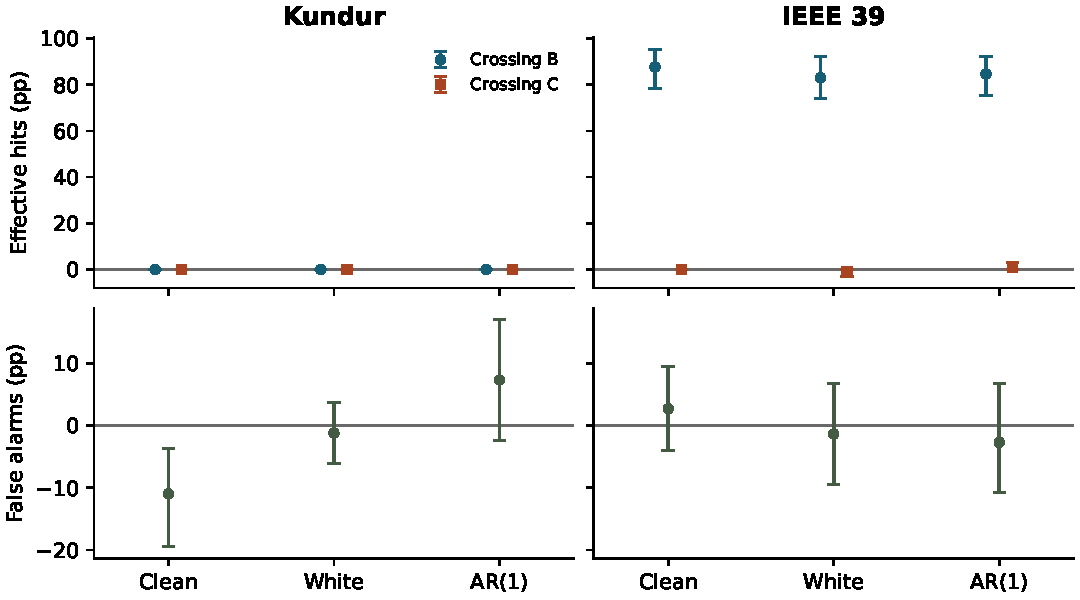
\includegraphics[width=.92\linewidth]{conditions.pdf}\caption{Full window minus endpoint on the new local test designs. Top panels show effective-hit gains for crossings at 400--680 ms (B) or at least 700 ms (C). Bottom panels show additional false alarms on safe designs. Points and bars give paired differences and event-clustered 95\% intervals.}\label{fig:conditions}\end{figure}

On IEEE 39 the endpoint predictor eventually alarmed on all 195 B variants, but only 24 met the lead requirement. The full window alarmed on 190 and each of those alarms met it. Median observed first-alarm times were 400 and 200 ms for endpoint and full window. In contrast, on Kundur both did so at 200 ms on every known B variant. Persistence eventually alarmed on all of those variants but missed their deadlines. This ceiling explains the zero observed Kundur gain over the trained endpoint and its large gain over persistence. IEEE 39 had no complete B trajectory among 49 B training designs or 65 B test designs. Local regressors learned suffix minima only from complete trajectories. The large observed B hit contrast therefore concerns timing on observed prefixes outside the B training-target support. It cannot verify nadir accuracy on those events. The supplement retains the earlier small numerical diagnostic alongside the full-frame recheck below.

Across clean, white and correlated noise respectively, IEEE 39 B hit gains were 87.69, 83.08 and 84.62 points. On Kundur the hit contrast stayed at zero across all three, but its additional false-alarm rate moved from $-10.98$ points on clean data to $+7.32$ on correlated noise. The within-event change of 18.29 [6.10, 30.49] points is an exploratory measurement interaction. Equal weighting conceals that change of sign.

On IEEE 39, the earliest B window fell in the highest quality-proxy bin on all 195 variants. At that decision the original switch always selected the endpoint expert. The separate ECGR scorer achieved 34/195 effective B hits, the switch 24/195, and quadratic regression features 19/195. On Kundur all three reached 252/252. The archive and these local results delimit representation choice by task, measurement and deadline.

\paragraph{Aligning lead and cost in time.} On the original IEEE 39 B cohort, the full-window policy achieved a median effective lead of 380 ms across its four opportunities, compared with 200 ms for the endpoint (medians among effective hits). Cumulative operating points compare the same two policies at the same final decision, without recalibration. At 200 ms the window gained 97.44 points while adding 18 false alarms per 222 safe variants. By 500 ms the endpoint had recovered some timely hits and generated additional false alarms of its own. The intervals in this sensitivity series resample common test-design IDs across solvers. The original within-stratum bootstrap is retained for the primary report. Table~\ref{tab:r2time} shows both sides of this timing trade-off.
\begin{table}[htbp]\centering\footnotesize\setlength{\tabcolsep}{4pt}
\caption{IEEE 39. W/E are full-window and endpoint counts with their common variant denominator in parentheses. Differences include paired physical-event 95\% bootstrap intervals. T and BE denote trapezoidal and backward Euler integration, with steps in ms. Finer settings are post hoc sensitivity checks with unchanged thresholds.}\label{tab:r2time}
\begin{tabular}{@{}llllll@{}}
\toprule Grid & Last ms & B: W/E ($n$) & Hit diff. (pp) & Safe: W/E ($n$) & FA diff. (pp) \\\midrule
10 T & 200 & 190/0 (195) & 97.44 [95.00, 99.46] & 19/1 (222) & 8.11 [4.57, 12.16] \\
10 T & 300 & 190/0 (195) & 97.44 [95.00, 99.46] & 22/8 (222) & 6.31 [2.95, 10.42] \\
10 T & 400 & 190/24 (195) & 85.13 [76.41, 92.38] & 24/14 (222) & 4.50 [0.44, 8.97] \\
10 T & 500 & 190/24 (195) & 85.13 [76.41, 92.38] & 27/28 (222) & -0.45 [-5.02, 4.35] \\
5 T & 200 & 194/0 (195) & 99.49 [98.28, 100.00] & 22/7 (222) & 6.76 [3.07, 10.50] \\
5 T & 500 & 194/15 (195) & 91.79 [83.97, 97.40] & 63/47 (222) & 7.21 [2.11, 12.50] \\
5 BE & 200 & 193/0 (195) & 98.97 [97.40, 100.00] & 17/8 (231) & 3.90 [0.51, 7.31] \\
5 BE & 500 & 193/18 (195) & 89.74 [81.54, 96.20] & 67/57 (231) & 4.33 [-0.94, 9.88] \\
2.5 T & 200 & 194/0 (195) & 99.49 [98.28, 100.00] & 27/12 (222) & 6.76 [2.44, 11.40] \\
2.5 T & 500 & 194/9 (195) & 94.87 [88.56, 99.46] & 102/65 (222) & 16.67 [10.93, 22.78] \\
\bottomrule\end{tabular}\end{table}
\paragraph{Training support and numerical sensitivity.} All 49 historical B training designs lacked a complete nadir target. At the first decision every one of the 195 B test endpoints was outside the marginal range of the fitted training pool. The endpoint ensemble mapped them to a single leaf signature and score. On the clean inputs the full-window ensemble produced seven signatures among 65 designs. Neither predictor attained an extreme of its training scores at this clean first decision. Thus a constant early endpoint score and later threshold crossings can coexist. These are diagnostics of piecewise-constant prediction outside observed feature support.
We reintegrated every IEEE 39 test design at both 5-ms settings and at 2.5 ms trapezoidal, including numerical failures and borderline leads. Each solver was evaluated against its own observed crossing and verified safe trajectories. The 500-ms B gain ranged from 89.74 to 94.87 points and the concurrent safe-event cost from 4.33 to 16.67 points. Of the three sensitivity settings, 0 met the two numerical limits on this dataset. None is a fresh confirmatory sample. 5 T classified 65 B and 74 safe designs. 5 BE classified 65 B and 77 safe designs. 2.5 T classified 65 B and 74 safe designs. Across the full IEEE 39 frame, the numbers of changed crossing strata were 0, 3, 0 for 5-ms trapezoidal, 5-ms backward Euler and 2.5-ms trapezoidal integration, respectively. At 2.5 ms the membership of all risk and safe strata matched the original. Nevertheless the window increased from 27 to 102 false alarms among 222 safe variants, while the endpoint increased from 28 to 65. This change cannot be explained by a change of denominator. Re-evaluating the same B designs with the original alarm times and new crossings leaves full-window hits at 190 and reduces endpoint hits from 24 to 9. With new alarms and original crossings the counts instead become 194 and 24. The additional four window hits therefore reflect changed first alarms, while the loss of fifteen timely endpoint hits reflects the shifted crossing relative to the 200-ms lead boundary. The supplementary material tracks stratum changes and contrasts the same physical IDs across integrators. The conditional B--C contrast also reflects the different perturbations and inertia values that produce those crossing times.

\paragraph{Revisiting incomplete original designs.} Kundur now has 201 known risk and 329 known safe designs out of 600. The updated T3 hit difference is 2.49 [1.16, 3.98] points and the false-alarm difference is -2.53 [-4.46, -0.51]. Allowing arbitrary outcomes on the remaining designs gives hit bounds [-23.99, 27.68] points. IEEE 39 now has 125 known risk and 475 known safe designs out of 600. The updated T3 hit difference is 26.40 [21.33, 31.73] points and the false-alarm difference is 0.98 [-1.12, 3.02]. Allowing arbitrary outcomes on the remaining designs gives hit bounds [26.40, 26.40] points. These identification limits describe possible completions of the planned series. Sampling intervals in brackets after point estimates describe variation among known outcomes. The original transfer figure retains its historical complete-case population.

\paragraph{Why first alarms change with the numerical clock.}
Each simulator used the same nominal measurement times. After the load step, the previous accepted state at the first decision was 9.90, 4.90 and 2.40 ms old in the 10-, 5- and 2.5-ms trapezoidal probes. The COI crossing label used the same held clock. Thus refinement changed both the integrated trajectory and the age of the observed state. Table~\ref{tab:r3clock} repeats the fixed policies with solver steps constrained to land on each reading time. Keeping the 10-ms native trajectories fixed and interpolating offline at the nominal grid changed the first alarm on 2/12 full-window and 1/12 endpoint probe variants. This diagnostic uses both bounding states; aligned reruns use only current and previously accepted states. The aligned backward-Euler run left 77 designs of unknown risk and yielded no complete safe design; its false-alarm rate is unidentified under the original termination flag. Rerunning all 320 designs with the last integration step landing exactly at 21 s restored 151 complete trajectories, including 77 previously unknown safe designs. The measured prefixes, crossing times and first alarms were unchanged; the corrected safe counts were 121 and 70 of 231 variants. Training and calibration still reflect the historical sampling procedure.
With grid-aligned readings the net safe-event cost was +28.38, +26.13, +26.13 and +26.13 points at 10, 5, 2.5 and 1.25 ms. Across the last two steps the largest change in either absolute false-alarm rate was 0.00 points. These are fixed-policy sensitivities on the same designs. Across the original 10- and 2.5-ms trapezoidal runs, 81 safe variants switched their full-window alarm outcome. All 81 changed leaf signature at their first discordant decision and retained the same reference value. For the endpoint, 51 switched, including 12 whose reference value also changed. The median maximum input-waveform change across those windows was 4.27 mHz for either method. Among the endpoint B variants, 15 lost timely status through a shifted crossing deadline with unchanged first-alarm timing. These distinct pathways explain why an earlier risk alarm can persist alongside unstable absolute false-alarm rates.
\begin{table}[htbp]\centering\small
\caption{IEEE 39 through 500 ms. Counts give full window/endpoint (variant denominator). Paired differences are in percentage points with design-clustered 95\% intervals. Held readings use the previous accepted solver state. Aligned integrations land on the observation clock. All rows use the historical fitted policies.}\label{tab:r3clock}
\resizebox{\linewidth}{!}{\begin{tabular}{llrrrr}\toprule
Readout & Scheme (ms) & Timely B & Difference & Safe alarms & Difference\\\midrule
held & 10 T & 190/24 (195) & 85.13 [76.41, 92.38] & 27/28 (222) & -0.45 [-5.02, 4.35] \\
held & 5 T & 194/15 (195) & 91.79 [83.97, 97.40] & 63/47 (222) & 7.21 [2.11, 12.50] \\
held & 5 BE & 193/18 (195) & 89.74 [81.54, 96.20] & 67/57 (231) & 4.33 [-0.94, 9.88] \\
held & 2.5 T & 194/9 (195) & 94.87 [88.56, 99.46] & 102/65 (222) & 16.67 [10.93, 22.78] \\
held & 1.25 T & 194/6 (195) & 96.41 [91.15, 100.00] & 113/62 (222) & 22.97 [15.49, 30.20] \\
aligned & 10 T & 195/6 (195) & 96.92 [91.94, 100.00] & 132/69 (222) & 28.38 [21.83, 35.42] \\
aligned & 5 T & 195/6 (195) & 96.92 [91.94, 100.00] & 122/64 (222) & 26.13 [19.05, 33.33] \\
aligned & 5 BE & 194/9 (195) & 94.87 [88.56, 99.46] & no eligible variants & unidentified \\
aligned & 5 BE (terminal fix) & 194/9 (195) & 94.87 [88.56, 99.46] & 121/70 (231) & 22.08 [15.24, 29.12] \\
aligned & 2.5 T & 195/6 (195) & 96.92 [91.94, 100.00] & 121/63 (222) & 26.13 [18.92, 33.33] \\
aligned & 1.25 T & 195/6 (195) & 96.92 [91.94, 100.00] & 121/63 (222) & 26.13 [18.92, 33.33] \\
\bottomrule\end{tabular}}\end{table}
\section{An independent support-stratified test}
The clock correction allowed us to ask whether the timing contrast survived when early-decline inputs could contribute complete training targets. A separate 36-design pilot sampled step size and inertia without using earlier test scores. The sampling rule retained safe, complete B, partial B and other complete risk cells. Before generating any new test trajectory we froze the sampling frame, fitted predictors, development offsets, calibration thresholds and analysis code. All new trajectories used the grid-aligned 1.25-ms trapezoid; the noise law, four decision times, suffix target and 200-ms lead were common to every predictor. We fitted endpoint and full-window trees with equal boosting budgets, and two standardized ridge regressions with the same penalty. The latter allow scores to vary beyond fitted feature ranges.
There were 180 training, 112 development, 180 calibration and 240 test designs. Of 80 B training designs, 59 supplied a complete suffix target. Test counts were 0 A, 111 B, 40 C, 89 safe and 0 unknown. At the first B decision the new endpoint tree used 21 distinct leaf signatures; the largest tied score accounted for 84/333 variants. Within the common training envelope the tree hit difference was +0.00 points [0.00, 0.00] across 263 B variants from 97 physical designs. The joint hit and cost criterion failed. Table~\ref{tab:supportnew} gives both representations and both model families.
The endpoint reached the timely-hit ceiling. Every resampled B design therefore contributed a zero paired difference. The resulting [0, 0] interval describes these observed pairs and cannot establish equivalence in a broader event population. These are independent parameter draws within the same IEEE 39 dynamic model. The new experiment supplies no additional physical network.
\par
\begin{table}[htbp]\centering\small
\caption{Independent support-stratified test through 500 ms (four cumulative opportunities). Counts are full window/endpoint (measurement-variant denominator). Inside requires every first-window coordinate in both representations to lie within its training range. The false-alarm columns refer to safe designs. Paired differences are in percentage points with 95\% physical-design bootstrap intervals.}\label{tab:supportnew}
\resizebox{\linewidth}{!}{\begin{tabular}{llrrrr}\toprule Family & Envelope & Timely B & Difference & Safe alarms & Difference\\\midrule
tree & all & 333/333 (333) & +0.00 [0.00, 0.00] & 61/33 (267) & +10.49 [2.53, 18.67] \\
tree & inside & 263/263 (263) & +0.00 [0.00, 0.00] & 60/32 (249) & +11.24 [2.98, 19.58] \\
tree & outside & 70/70 (70) & +0.00 [0.00, 0.00] & 1/1 (18) & +0.00 [-17.39, 15.39] \\
ridge & all & 333/333 (333) & +0.00 [0.00, 0.00] & 55/27 (267) & +10.49 [3.90, 17.27] \\
ridge & inside & 263/263 (263) & +0.00 [0.00, 0.00] & 54/26 (249) & +11.24 [4.54, 18.34] \\
ridge & outside & 70/70 (70) & +0.00 [0.00, 0.00] & 1/1 (18) & +0.00 [-17.39, 15.39] \\
\bottomrule\end{tabular}}\end{table}
\par

Across all safe designs, the full-window tree issued more alarms under each measurement law. The excess was 11.24 points for clean readings, 8.99 for white noise and 11.24 for AR(1). The white-noise interval included zero. The ridge contrasts had the same sign in all three laws. Outside the common coordinate ranges, there were only nine safe variants per noise law and none under clean readings: both families added one white-noise alarm and avoided one AR(1) alarm. Their pooled zero therefore hides opposite signs in small cells. Supplementary Tables~S33 and S34 give both absolute operating points and paired intervals.

\section{Discussion}
A matched endpoint leaves physically meaningful variation in the subsequent nadir. The aggregate confirmation establishes a corresponding increment in effective warnings under the tested noise mixture and threshold procedure. The common proxy itself depends on in-window roughness. This makes the comparison deliberately stricter than a comparison with an untrained persistence forecast, while leaving open which individual interior samples carry the increment. Equal depth and boosting budget likewise control learner design without guaranteeing identical effective degrees of freedom.

The fixed 200-ms deadline had different operational meanings across models. In the aggregate confirmation 241 of 405 risk events could no longer be warned by the last window. In the original completed network tests the earliest crossings were 1.32 s (Kundur) and 1.74 s (IEEE 39). Every one of the four decision times could therefore meet the lead requirement. The original transfer evidence concerns distinguishing later-crossing risk events from safe events using early observations. It provides no direct test of network events whose deadline expires within the observation window. Moreover, the quality proxy is sensitive to physical waveform roughness: all clean Kundur windows were assigned to the highest bin and no clean original IEEE 39 window occupied the lowest bin, whereas all 9,600 clean aggregate window visits occupied the lowest bin. A bin label cannot be interpreted as a transportable estimate of sensor noise. The source and target experiments differ in parameter support, dynamic structure, and in the relationship between the measured signal and the risk label. Changing all three precludes a causal assignment to any one physical factor. The supplement reports the original opportunity fractions and deadline-aware score rankings.

Within each measurement law we also examined how much the training suffix minima varied among 15 nearby endpoints at the first decision. Kundur had 0 and 84 clean B events below or at versus above its development median spread, contributing 0 and 0 net full-window hits. IEEE 39 had 65 and 0 clean B events below or at versus above its development median spread, contributing 57 and 0 net full-window hits. Unequal support, labelled training neighbours and the association of disturbance severity with crossing time limit this exploratory comparison. It does not validate an online selection rule.

Results concern a realised calibration set and a scalar readout. The simulator assumes a known disturbance origin and synthesised measurement noise. It does not include an end-to-end detection, communications or actuation chain. All simulations on a given network share its equations and dynamic data. In particular, hundreds of disturbances do not represent hundreds of independent power systems.

\section{Conclusion}
In the independent IEEE 39 test, the full-window and endpoint representations reached the observed timely-hit ceiling with both tree and ridge predictors (333/333 B variants each). This leaves their relative hit rates in a broader population unresolved. Through 500 ms, the full-window tree triggered on 61/267 safe variants versus 33/267 for the endpoint, a difference of 10.49 points [2.53, 18.67]. The joint criterion failed. A difference in safe alarms persisted within the common training ranges, while the small outside groups gave opposite signs under white and correlated noise.

The historical 85.13-point B gain compared fixed policies under held readout, with every first-window B endpoint beyond its training range. The endpoint tree eventually detected all 195 B variants, but only 24 alarms met the deadline. Held-readout operating points failed to converge over the tested refinements. At the aligned 1.25-ms step, the full-window and endpoint policies alarmed on 121/222 (54.50\%) and 63/222 (28.38\%) safe variants. The aligned audit retained historical training, development and calibration. The fresh study changed the sampling frame and fitted policies together, leaving the contributions of physics, readout and extrapolation to the historical contrast unidentified.

Under the specified aggregate model, noise mixture, frozen thresholds and sampled population, the short window added predictive information about the nadir and increased effective warnings. The quadratic result limits claims for specialised shape compression. On the original transfer series, aggregate thresholds gave no alarms on either network and missing Kundur outcomes still permit either sign of the planned-population hit difference. The deadline study failed the joint criterion on both networks. These simulations with known disturbance origin and synthetic measurements establish neither a common network advantage nor field performance.
\paragraph{Data and code availability.}
The r4 release provides the independent count audit, aligned per-window comparisons, source fingerprints, and executable replay and rebuild commands. Its companion r3 archive preserves the trajectories, numerical logs, fitted models and unrounded binary thresholds. The supplement documents their use.
\footnotesize\begin{thebibliography}{9}\setlength{\itemsep}{1pt}
\bibitem{sfr} P.M. Anderson, M. Mirheydar. A low-order system frequency response model. \emph{IEEE Transactions on Power Systems}, 1990, 5, 720--729. \href{https://doi.org/10.1109/59.65898}{doi: 10.1109/59.65898}.
\bibitem{liu} Liu Liu, Weidong Li, Yu Ba, Jiakai Shen, Cuicui Jin, Kerui Wen. An Analytical Model for Frequency Nadir Prediction Following a Major Disturbance. \emph{IEEE Transactions on Power Systems}, 2020, 35, 2527--2536. \href{https://doi.org/10.1109/tpwrs.2019.2963706}{doi: 10.1109/tpwrs.2019.2963706}.
\bibitem{early} Dimitrios Zografos, Tin Rabuzin, Mehrdad Ghandhari, Robert Eriksson. Prediction of Frequency Nadir by Employing a Neural Network Approach. \emph{2018 IEEE PES Innovative Smart Grid Technologies Conference Europe (ISGT-Europe)}, 2018, 1--6. \href{https://doi.org/10.1109/isgteurope.2018.8571581}{doi: 10.1109/isgteurope.2018.8571581}.
\bibitem{polynomial} Hongxin Li, Lisen Wang, Sirui Qi, Ziqiang Wang, Yanting Wang, Shichen Zhou, Wenwei Zheng. Power system frequency nadir prediction based on data-driven and power-frequency polynomial fitting. \emph{Frontiers in Energy Research}, 2024, 12, article 1501181. \href{https://doi.org/10.3389/fenrg.2024.1501181}{doi: 10.3389/fenrg.2024.1501181}.
\bibitem{transfer} Jian Xie, Wei Sun. A Transfer and Deep Learning-Based Method for Online Frequency Stability Assessment and Control. \emph{IEEE Access}, 2021, 9, 75712--75721. \href{https://doi.org/10.1109/access.2021.3082001}{doi: 10.1109/access.2021.3082001}.
\bibitem{nadir25} Manuel Jesús Jiménez-Navarro, Jose Miguel Riquelme-Dominguez, Manuel Carranza-García, Francisco M. González-Longatt. A real-time machine learning-based methodology for short-term frequency nadir prediction in low-inertia power systems. \emph{Neurocomputing}, 2025, 626, article 129583. \href{https://doi.org/10.1016/j.neucom.2025.129583}{doi: 10.1016/j.neucom.2025.129583}.
\bibitem{event} Nesime Tatbul, Tae Jun Lee, Stan Zdonik, Mejbah Alam, Justin Gottschlich. Precision and Recall for Time Series. \emph{Advances in Neural Information Processing Systems 31}, 32nd Conference on Neural Information Processing Systems, Curran Associates, Inc., 2018, pp.~1920--1930.
\bibitem{calibration} Xin Tong, Yang Feng, Jingyi Jessica Li. Neyman-Pearson classification algorithms and NP receiver operating characteristics. \emph{Science Advances}, 2018, 4(2), eaao1659. \href{https://doi.org/10.1126/sciadv.aao1659}{doi: 10.1126/sciadv.aao1659}.
\bibitem{andes} Hantao Cui, Fangxing Li, Kevin Tomsovic. Hybrid Symbolic-Numeric Framework for Power System Modeling and Analysis. \emph{IEEE Transactions on Power Systems}, 2021, 36, 1373--1384. \href{https://doi.org/10.1109/tpwrs.2020.3017019}{doi: 10.1109/tpwrs.2020.3017019}.
\end{thebibliography}
\end{document}
